\documentclass[../../master_thesis_np.tex]{subfiles}
\graphicspath{{./imgs/}}

\begin{document}
\chapter[Interaction Implementation]{Implementation of interactions in simulations}
\label{chap:int_impl}
	\section{Previous Developments}
	All the code work in this thesis is built on top of an existing code written and used in Microscale Robotics Lab, which can be found in repository \cite{sharma_simulations_2023}. Existing code performed simulations on 2D active Brownian particles moving in open or closed boundary featuring confinement. The interactions among these particles were steric hard sphere correction, which are enough to study clustering, MIPS and boundary accumulation. The hard sphere correction follows algorithm \ref{alg:hardsphere} according to \cite{callegari_numerical_2019}.

	\begin{algorithm}[htp]
		\caption{The hard sphere correction algorithm} \label{alg:hardsphere}	
		\begin{algorithmic}[1]
			\ForAll{couples of particles $\{i, j\}$}
			\State{$d_{i,j} \gets d(\mathbf{r}_{i}, \mathbf{r}_{j})$} \Comment{$d\left(\cdot,\cdot \right)$ is the Euclidean distance}

			\State{$\mathbf{n}_{i,j} = \left(\mathbf{r}_{i}-\mathbf{r}_{j}\right)/d_{i,j}$}
			\If{$d_{i,j} < 2R$}\Comment{$R$ is the particles' radius}
			\State{$\mathbf{r}_i \gets \mathbf{r}_i - \mathbf{n}_{i,j}d_{i,j}/2$}
			\State{$\mathbf{r}_j \gets \mathbf{r}_i - \mathbf{n}_{j,i}d_{i,j}/2$}
			\EndIf
			\EndFor
		\end{algorithmic}
		\end{algorithm}

		\begin{figure}[htp]
			\centering
			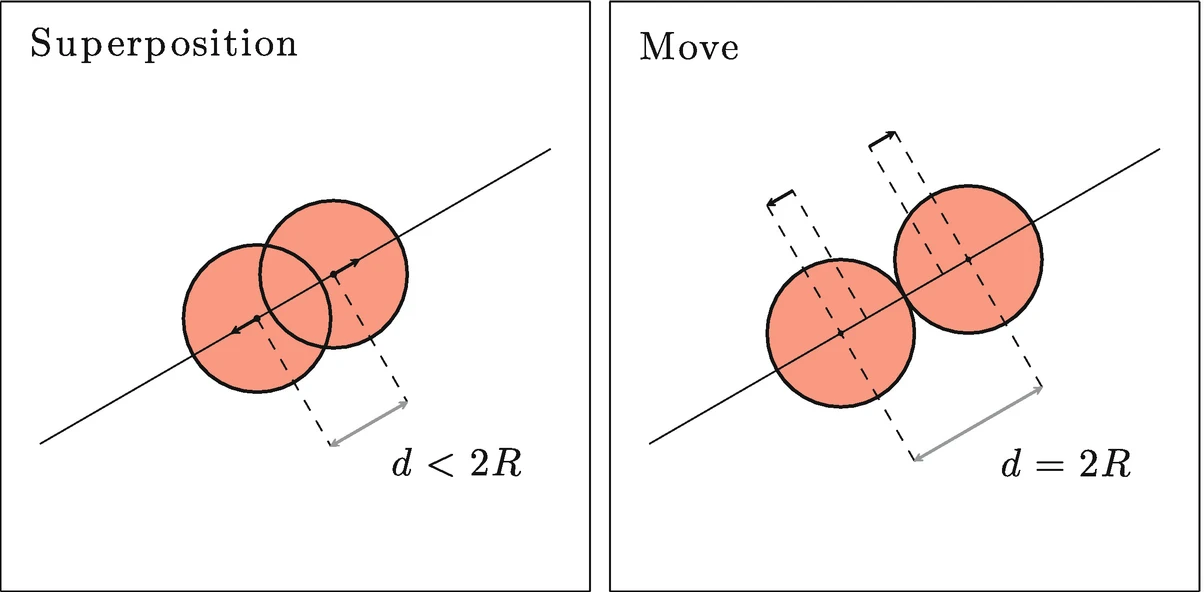
\includegraphics[width = 0.7\textwidth]{callegari_volpe_2019_hardsphere.png}
			\label{fig:hardsphere}
			\caption{ \cite{callegari_numerical_2019}}
		\end{figure}

	This operation involves calculating the distance matrix of a set of $n$ particles, i.e.~computing $n^2$ distances. Being a $O(n^2)$ algorithm, this kind of correction can become computationally demanding, especially for high density and velocity systems, where collisions and clustering are more likely to happen.
	
	Since hard sphere corrections were implemented to study ABPs in confinement rather than open periodic boundary, this interaction could not take periodicity into account leading to possible superpositions at the simulation box borders.
	
	Finally, let us explain the physics behind this kind of correction. Moving superimposing particles of just the right amount to keep them in contact may seem a somehow strong assumption, since it is simulating a perfectly inelastic collision. Actually, if one wanted to simulate balls moving on a pool table, where macroscopic Newtonian dynamics take place, it would be easy to state whether collisions are elastic or not (in the mentioned case, yes). Here we can exploit what was found by, among others \citeauthor{singh_pair_2024} in \cite{singh_pair_2024}, where the contact time for Janus colloids was characterized, in different collision scenarios. They found contact times of the order of $\sim \text{s}$, similarly to what is often observed in Microscale Robotics Lab, motivating the choice of a completely inelastic collision, where adhesion forces keep particles together after the impact. 
	
	\section{Model}
	There are several examples in literature of aligning interactions applied to ABPs systems. Most of them involve applying a torque which explicitly depends on the difference between the orientation angle of the two interacting particles; some of them have a constant torque which is applied to particles closer than a certain distance. To the best of our knowledge, nobody tried before to implement an interaction in the system which unifies the central force and the torque. 
	
	The model used in this thesis aims to keep a minimal amount of parameters while coupling positions and orientations of interacting particles, actually using only one more parameter than a force-only model.
	
	If one was to apply a central force to a set of particles, the way would be computing a distance matrix between the positions of particles' centers, calculating the absolute value of the force with a function $F(\abs{r})$, and applying it to particle positions, splitting the two components (we are simulating in 2D).
	
	Here every particle is identified by two positions: its center of mass, which lies in its geometric center, and an interaction center, which is translated with respect to the center of mass of an amount $\alpha R$ in the direction of self-propulsion, so that the off center position of each particle writes:
	\begin{equation}
		\vec{x}_{oc} = \vec{x}_{cm} + \alpha R 
		\begin{pmatrix}
			\cos(\theta)\\
			\sin(\theta)
		\end{pmatrix}
	\end{equation}
	where $\theta$ is the self-propulsion direction and $-1 < \alpha < 1$. This way distances,and hence forces, are computed starting from off center positions; applying forces to the same positions results both in a translation effect and in a torque applied to the particle, coupling the two degrees of freedom.
	
	The idea is to take into account the underlying particle's asymmetry in simulations. It is a fact that the two faces of a Janus particles have different physical and chemical properties, which make them interact differently depending on the angle between their orientations and the line connecting their centers \cite{singh_pair_2024}. This can be due to a plethora of effects like chemical gradients, electrical forces or hydrodynamics, but this model takes only the asymmetry along with standard potentials

	\section{Steric Interactions}
	\subsection{All to All}
	\subsection{Range}
	\section{Aligning Interactions}

\end{document}